\documentclass{beamer}
\input{../style/cours-style.sty}

% Title
\title[JavaScript]{JavaScript Frontend - B1 Web et Multimédia}
\author{Christophe Brun}
\institute{My Digital School}
\beamertemplatenavigationsymbolsempty

\titlegraphic{
    \bigbreak
    
\includegraphics[width=5cm]{image/mds-logo}
    \bigbreak
    L’école des métiers du digital
    \bigbreak
}

\begin{document}

    \begin{frame}
        \titlepage
        \bigbreak
        \centering
        \url{https://github.com/My-Digital-School-by-PapIT/frontend-JS}
    \end{frame}


    \section{Table des matières}\label{sec:toc}

    \begin{frame}{Table des matières}
        \begin{tiny}
            \begin{multicols}{1}
                \tableofcontents
            \end{multicols}
        \end{tiny}
    \end{frame}


    \section{Programme du module}\label{sec:programme-du-module}

    \begin{frame}{JavaScript Frontend}{Objectifs des 6 jours}
        \begin{columns}
            \column{0.7\textwidth}
            \begin{scriptsize}
                \begin{itemize}
                    \item Distinguer les différentes parties prenantes du web (protocol de communication, navigateur, serveur, \textit{etc}).
                    \item La syntaxe JavaScript.
                    \item La Window API, manipulation de DOM.
                    \item Intéragir avec une API depuis le frontend.
                \end{itemize}
            \end{scriptsize}
            \column{0.3\textwidth}
            
\includegraphics[width=4cm]{image/js-surfing}
        \end{columns}
    \end{frame}


    \section{Introduction}\label{sec:introduction}

    \begin{frame}{Formateur sur Linux}{Christophe Brun, conseil en développement informatique}

        \begin{columns}
            \column{0.7\textwidth}
            \begin{itemize}
                \item Développeur freelance (Python, Java, CoBOL) et data at scale.

                \item 7 ans de conseil en développement au sein d'SSII~.

                \item 7 ans de conseil en développement en indépendant, \href{https://papit.fr}{PapIT}.

                \item Passionné~!
                \bigbreak
                \begin{columns}
                    \column{0.5\textwidth}
                    \centering
                    
\includegraphics[width=3cm]{image/logo-uppa}
                    \column{0.5\textwidth}
                    \centering
                    
\includegraphics[width=3cm]{image/logo-universite-bordeaux}
                \end{columns}
            \end{itemize}
            \column{0.3\textwidth}
            \centering
            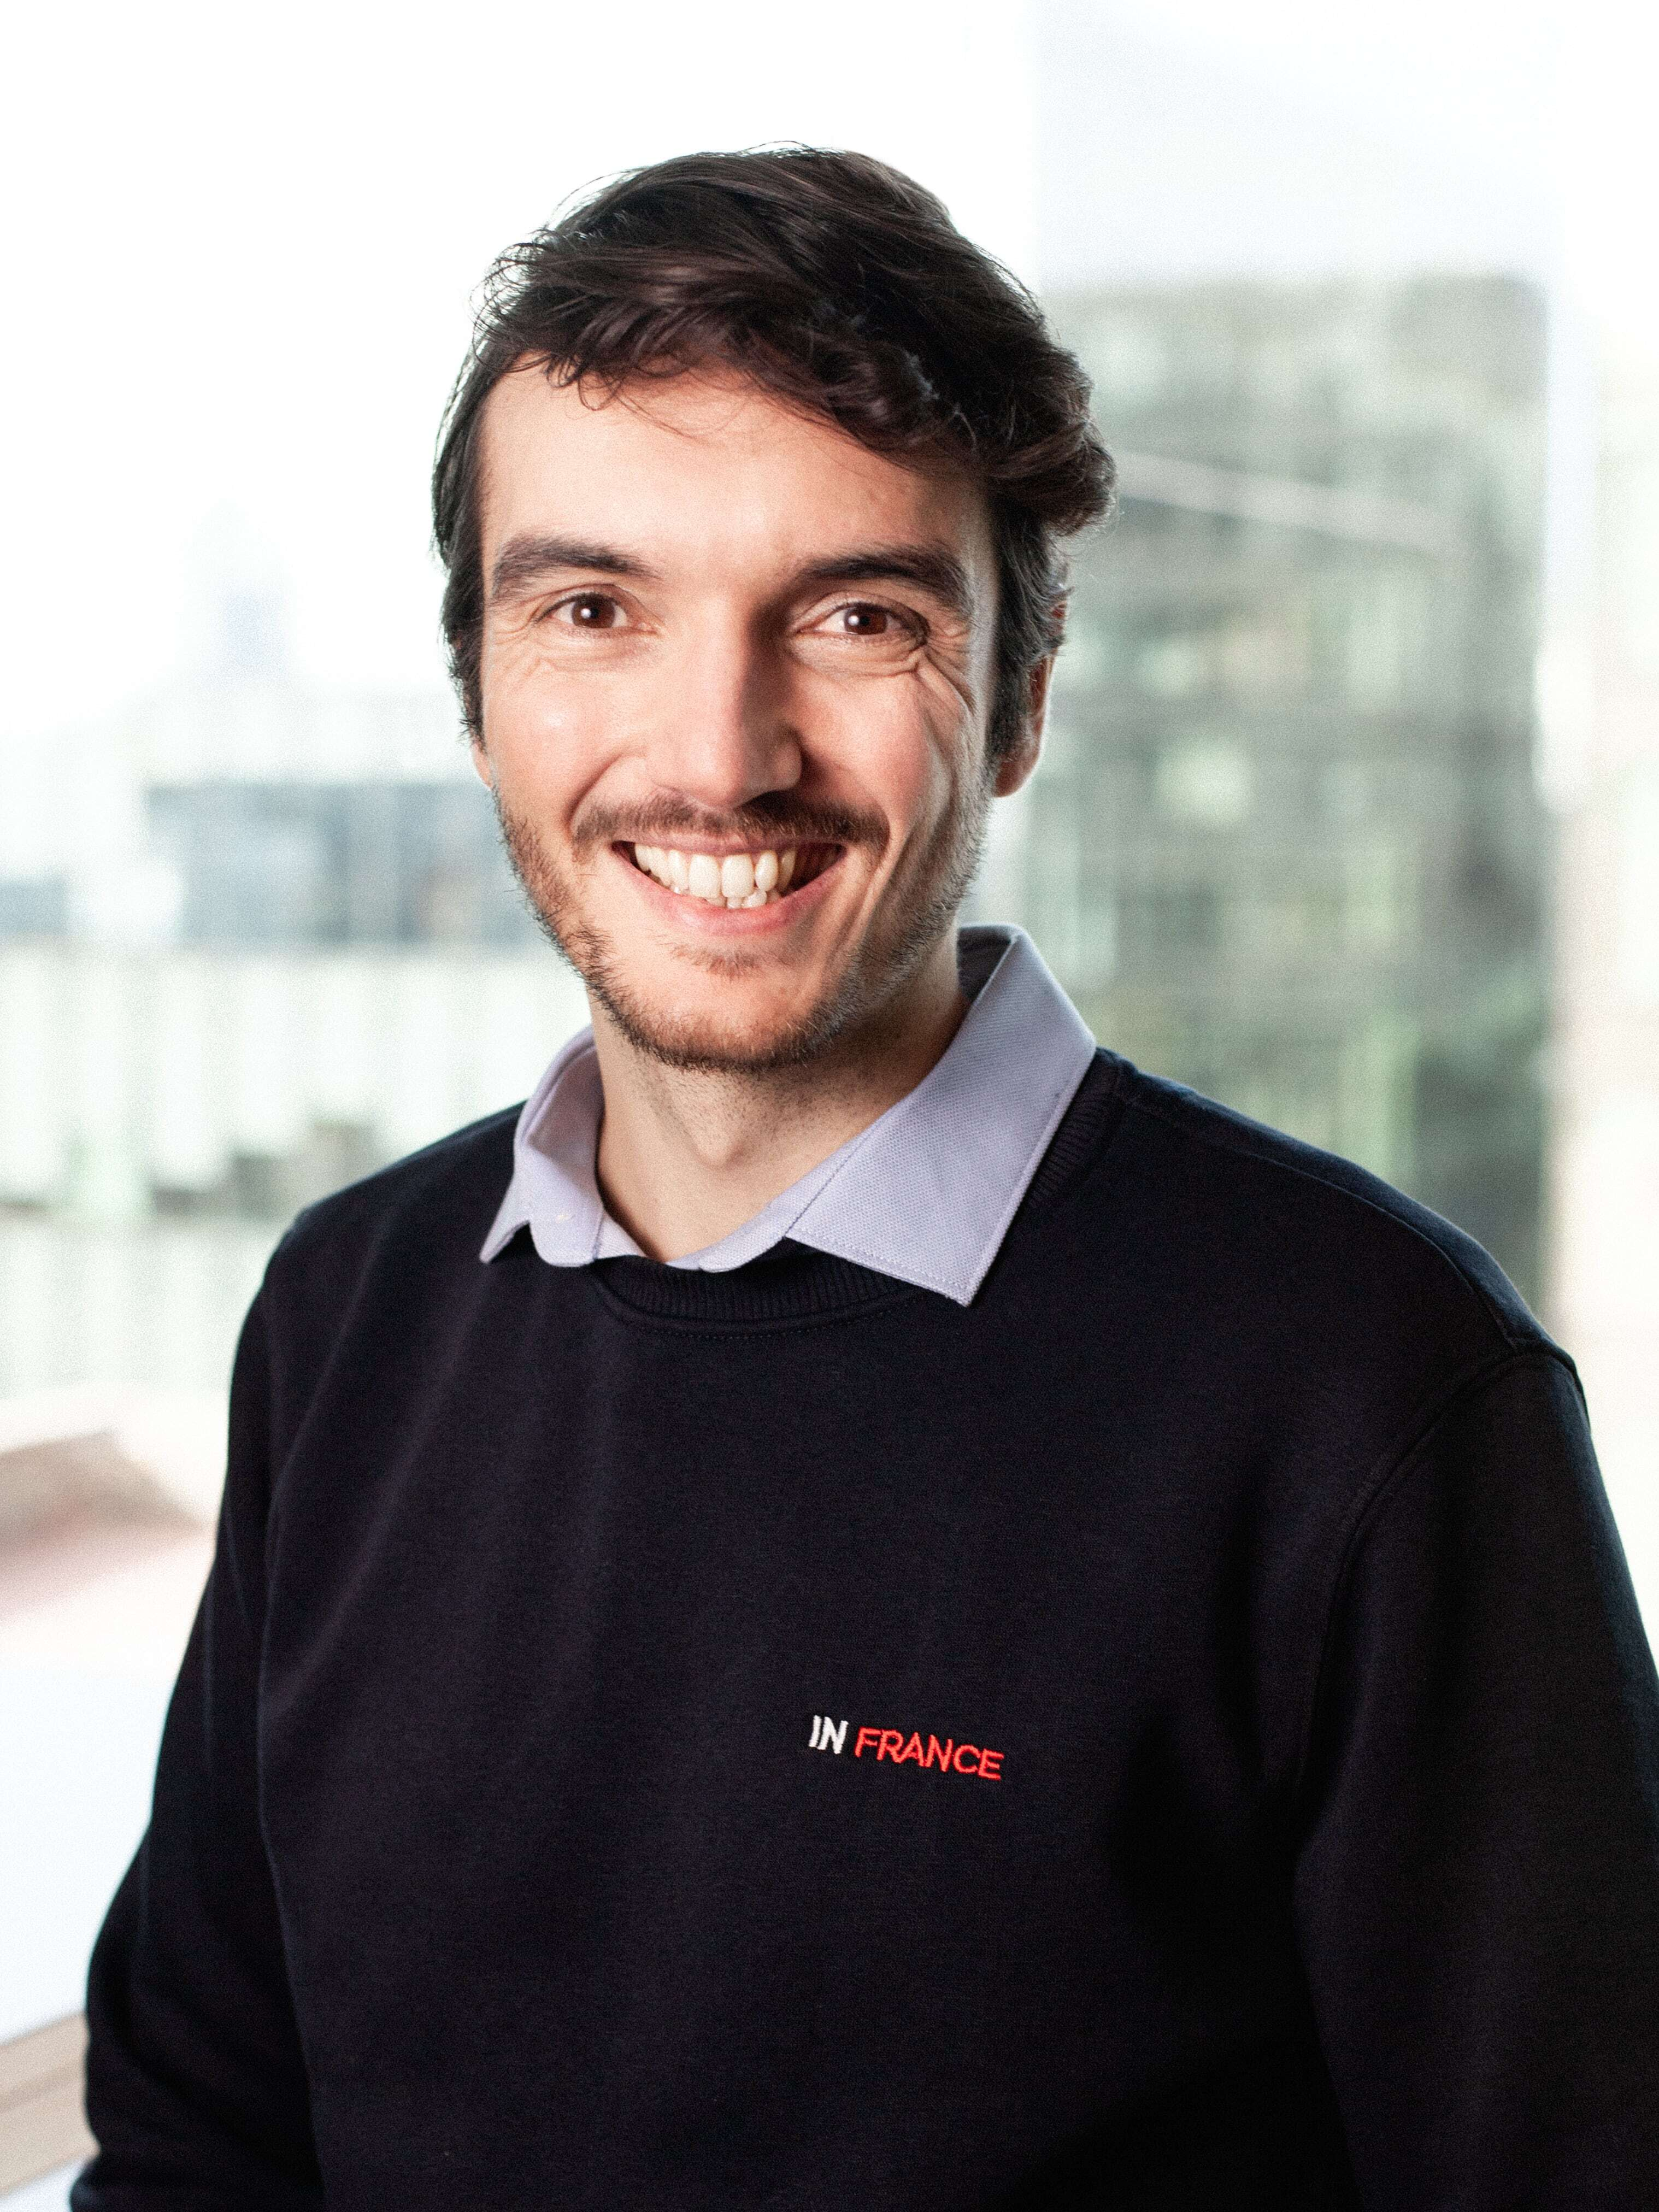
\includegraphics[width=5cm]{image/trombine-christophe}
        \end{columns}
    \end{frame}


    \section{Les ressources du Web}\label{sec:ressources}

    \begin{frame}{Les ressources du Web}{Dvisions en briques}
        \begin{columns}
            \column{0.6\textwidth}
            1 des 4 règles pour la direction de l'esprit de Descartes~: \textquote{Diviser chacune des difficultés que j'examinerais, en autant de parcelles qu'il se pourrait et qu'il serait requis pour les mieux résoudre.}.
            \column{0.4\textwidth}
            \centering
            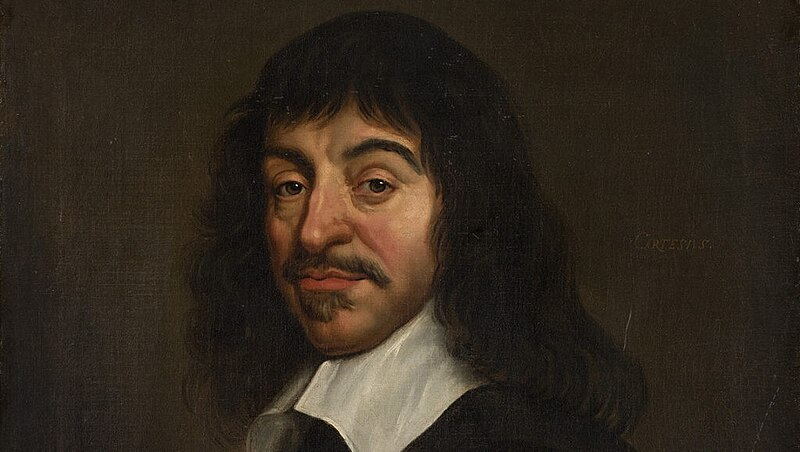
\includegraphics[width=6cm]{image/Descartes}
        \end{columns}
    \end{frame}

    \begin{frame}{Les ressources du Web}{Analyse des composants}
        \centering
        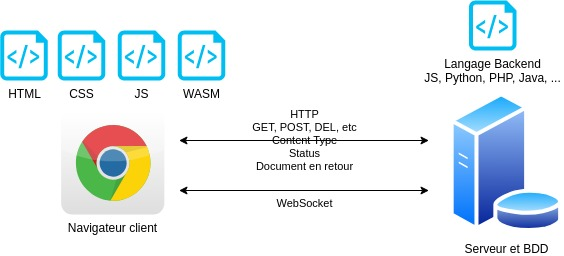
\includegraphics[width=11cm]{image/web-stakeholders.drawio}
    \end{frame}


    \section{Le web statique}\label{sec:static}

    \begin{frame}{Le web statique}
        Une des premières options pour un site web est donc d'être statique.

        Suite à une requête sur une URL (adresse dans le navigateur), le serveur nous envoie une page HTML pour la donnée avec du CSS pour le style.
        \bigbreak
        Il n'y a pas d'interaction avec le serveur, le contenu est figé, on peut juste passer à une autre page grâce à une ancre \lstinline{<a href="...">...</a>}.
        \bigbreak
        \centering
        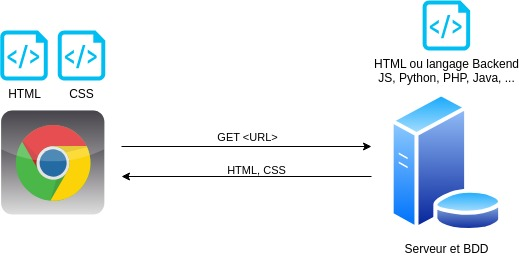
\includegraphics[width=8cm]{image/web-static}
    \end{frame}

    \begin{frame}[fragile]{Les ressources du Web}{Analyse des composants, exercice \execcounterdispinc{}}
        \begin{itemize}
            \item Installer Python 3.
            \item Installer un IDE de développement Web comme WebStorm.
            \item Lancer un serveur HTTP avec la commande dans le répertoire du cours~:
            \begin{lstlisting}[language=bash]
python3 -m http.server
            \end{lstlisting}
            \item Naviguer à l'adresse indiquée.
            \item Modifier le fichier \lstinline{index.html} pour ajouter un lien vers une page HTML développée par vos soins avec votre nom et une photo de vous.
            \item Rafraichir la page et vérifier que la modification est fonctionnelle.
        \end{itemize}
    \end{frame}

    \section{Le web dynamique}\label{sec:Dynamic}

    \section{Licence CC}\label{sec:licence}

    \begin{frame}{Licence}{Licence Creative Commons}
        Support de cours sous licence Creative Commons BY-NC-ND~.
        \bigbreak
        Vous pouvez donc, partager, copier, distribuer le document.
        \bigbreak
        Attribution requise à PapIT SASU - Pas d’utilisation commerciale - Pas de modification
        \bigbreak
        \centering
        
\includegraphics[width=5cm]{image/by-nc-nd-logo}
    \end{frame}


\end{document}
